%% Template para dissertação/tese na classe UFPEthesis
%% versão 0.9.2
%% (c) 2005 Paulo G. S. Fonseca
%% www.cin.ufpe.br/~paguso/ufpethesis

%% Carrega a classe ufpethesis
%% Opções: * Idiomas
%%           pt   - português (padrão)
%%           en   - inglês
%%         * Tipo do Texto
%%           bsc  - para monografias de graduação
%%           msc  - para dissertações de mestrado (padrão)
%%           qual - exame de qualificação doutorado
%%           prop - proposta de tese doutorado
%%           phd  - para teses de doutorado
%%         * Mídia
%%           scr  - para versão eletrônica (PDF) / consulte o guia do usuario
%%         * Estilo
%%           classic - estilo original à la TAOCP (deprecated)
%%           std     - novo estilo à la CUP (padrão)
%%         * Paginação
%%           oneside - para impressão em face única
%%           twoside - para impressão em frente e verso (padrão)
\documentclass[bsc]{ufpethesis}

%% Preâmbulo:
%% coloque aqui o seu preâmbulo LaTeX, i.e., declaração de pacotes,
%% (re)definições de macros, medidas, etc.

\usepackage{indentfirst}
\usepackage{setspace}
\usepackage{url}
\usepackage{scrextend}
\addtokomafont{labelinglabel}{\sffamily}
\usepackage{suffix}
\usepackage[withpage]{acronym} % optional command: printonlyused

\onehalfspacing

%% Identificação:

% Universidade
% e.g. \university{Universidade de Campinas}
% Na UFPE, comente a linha a seguir
%%\university{Universidade Federal de Pernambuco}

% Endereço (cidade)
% e.g. \address{Campinas}
% Na UFPE, comente a linha a seguir
%%\address{<CIDADE DA IES>}

% Instituto ou Centro Acadêmico
% e.g. \institute{Centro de Ciências Exatas e da Natureza}
% Comente se não se aplicar
\institute{Centro de Tecnologia e Geociências}

% Departamento acadêmico
% e.g. \department{Departamento de Informática}
% Comente se não se aplicar
\department{Departamento de Eletrônica e Sistemas}

% Programa de pós-graduação
% e.g. \program{Pós-graduação em Ciência da Computação}
\program{Bacharelado em Engenharia Eletrônica}

% Área de titulação
% e.g. \majorfield{Ciência da Computação}
\majorfield{Engenharia Eletrônica}

% Título da dissertação/tese
% e.g. \title{Sobre a conjectura $P=NP$}
\title{Iluminação de LED controlada pela internet}

% Data da defesa
% e.g. \date{19 de fevereiro de 2003}
\date{<DATA DA DEFESA>}

% Autor
% e.g. \author{José da Silva}
\author{Rafael Moreira Queiroz}

% Orientador(a)
% Opção: [f] - para orientador do sexo feminino
% e.g. \adviser[f]{Profa. Dra. Maria Santos}
\adviser{Gilson Jerônimo da Silva Junior}

% Orientador(a)
% Opção: [f] - para orientador do sexo feminino
% e.g. \coadviser{Prof. Dr. Pedro Pedreira}
% Comente se não se aplicar
%\coadviser{NOME DO(DA) CO-ORIENTADOR(A)}

%% Inicio do documento
\begin{document}

%%
%% Parte pré-textual
%%
\frontmatter

% Folha de rosto
% Comente para ocultar
\frontpage

% Portada (apresentação)
% Comente para ocultar
\presentationpage

% Dedicatória
% Comente para ocultar
\begin{dedicatory}
    Dedico este trabalho a todos que o tornaram possível.
\end{dedicatory}

% Agradecimentos
% Se preferir, crie um arquivo à parte e o inclua via \include{}
\acknowledgements
    Agradeço primeiramente a Deus por sua graça e luz em minha vida, aos meus pais Adelmo e Aparecida e a minha irmã Laura por todo o apoio, amor e compreensão, à minha namorada Mirla por estar sempre ao meu lado frente a todas as dificuldades, aos meus queridos amigos Paulo, Felipe, Samuel e Matheus, e ao meu orientador Prof. Gilson Jerônimo Junior.

% Epígrafe
% Comente para ocultar
% e.g.
%  \begin{epigraph}[Tarde, 1919]{Olavo Bilac}
%  Última flor do Lácio, inculta e bela,\\
%  És, a um tempo, esplendor e sepultura;\\
%  Ouro nativo, que, na ganga impura,\\
%  A bruta mina entre os cascalhos vela.
%  \end{epigraph}
\begin{epigraph}{Abraham Lincoln}
Não sou obrigado a vencer, mas tenho o dever de ser verdadeiro. Não sou obrigado a ter sucesso, mas tenho o dever de corresponder à luz que tenho.
\end{epigraph}

% Resumo em Português
% Se preferir, crie um arquivo à parte e o inclua via \include{}
\resumo
A iluminação de LED apresenta algumas vantagens diante das tradicionais iluminações fluorescentes e incandescentes. Lâmpadas ou fitas de LED são em geral mais eficientes, compactas e oferecem vantagens como variedade de cores em comparação às variantes tradicionais de iluminação e por isso vêm sendo utilizadas tanto em iluminação pública como em decoração e em pequenos dispositivos. A facilidade de controlar sua intensidade por meio do rápido chaveamento de sua potência é outro atrativo, principalmente quando se trata do uso de microcontroladores conectados à internet. Este trabalho apresenta uma implementação de um sistema de iluminação com fita de LEDs brancos controlada pelo sistema embarcado "ESP-8266" por meio da troca de dados pela internet com um aplicativo móvel por meio do protocolo de internet "MQTT" com a capacidade de ligar, desligar, arbitrar a intensidade da fita no modo manual ou ter a intensidade controlada automaticamente. Serão feitas medições do consumo do sistema para demonstrar a capacidade de economia de energia do sistema proposto.

% Palavras-chave do resumo em Português
\begin{keywords}
    Iluminação, LED, MQTT, ESP8266
\end{keywords}

% Resumo em Inglês
% Se preferir, crie um arquivo à parte e o inclua via \include{}
\abstract
Led illumination holds some advantages on fluorescent and incandescent forms of illumination. LED lamps or strips are, in general more efficient, compact and have features like color variety when compared to those other forms of illumination and that's why they are utilized on public lighting, decoration or on small gadgets. Ease of controlling its intensity by fastly keying its power source is an important feature when it comes to the use of microcontrollers like those connected to the internet. This work demonstrates an implementation of a lighting system with a white LED strip controlled by the embedded system "ESP-8266"  by means of data exchange on the internet with a mobile application with the MQTT internet protocol and it has the capability of turning on, off, setting the led strip's intensity or even setting the automatic intensity mode. Measurements will be taken in order to demonstrate the energy saving capability of this proposed system. 
% Palavras-chave do resumo em Inglês
\begin{keywords}
    Illumination, LED, MQTT, ESP8266
\end{keywords}

% Sumário
% Comente para ocultar
\tableofcontents

% Lista de figuras
% Comente para ocultar
\listoffigures

% Lista de tabelas
% Comente para ocultar
\listoftables

\chapter*{Lista de Siglas}
\begin{acronym}[MQTT]
    \acro{IEEE}{\textit{Institute of Electrical and Electronics Engineers}}
    \acro{IoT}{\textit{Internet of Things}}
    \acro{IP}{\textit{Internet Protocol}}
    \acro{LDR}{\textit{Light Dependent Resistance}}
    \acro{LED}{\textit{Light Emitting Diode}}
    \acro{MAC}{\textit{Media Access Control}}
    \acro{MQTT}{\textit{Message Queue Telemetry Transport}}
    \acro{PID}{Proporcional Integral Derivativo}
    \acro{PWM}{\textit{Pulse Width Modulation}}
    \acro{QoS}{\textit{Quality of Service}}
    \acro{SoC}{\textit{System on Chip}}
    \acro{TCP}{\textit{Transmission Control Protocol}}
    \acro{WiFi}{\textit{Wireless Fidelity}}
\end{acronym}

%%
%% Parte textual
%%
\mainmatter

% É aconselhável criar cada capítulo em um arquivo à parte, digamos
% "capitulo1.tex", "capitulo2.tex", ... "capituloN.tex" e depois
% incluí-los:
\chapter{Introdução}

O termo "Internet das Coisas" \space vem sendo usado extensivamente nos últimos anos e isso se deve ao fato, em conjunto com outros como "inteligência artificial", "\textit{Big Data}" \space e "computação em nuvem", de ser protagonista de uma latente revolução industrial, da informação e até da tecnologia de forma geral \cite{iot-future}. A possibilidade de ter dispositivos conectados à internet que podem ser controlados remotamente, que podem colher dados que são processados, analisados e usados para tornar processos cada vez mais eficientes e lucrativos tem movimentado um grande mercado em todo o mundo e promete continuar sua expansão \cite{iot-future}. 

Existem certos padrões de comportamento do público consumidor e da indústria diante de  tecnologias emergentes que são caracterizados por descoberta e discussão inicial, difusão entre adotadores precoces e por fim, uso extensivo. Pesquisas indicam que as barreiras iniciais à adoção da "Internet das Coisas" \space vêm sendo quebradas e a nova tecnologia está sendo encontrada não apenas em novas empresas (\textit{startups}) mas também têm atraído atenção da indústria de grande porte \cite{forbes}. 
%referencia da forbes 
%www.forbes.com/sites/louiscolumbus/2018/08/16/iot-market-predicted-to-double-by-2021-reaching-520b/

Outra forte tendência é o uso de diodos emissores de luz (LED) com a finalidade de iluminação tanto para ambientes abertos quanto para ambientes fechados, que já eram usados em produtos eletroeletrônicos e equipamentos sinalizadores como lâmpadas de emergência e semáforos. Há alguns anos a tecnologia já era estudada como solução para iluminação mas devido a seu custo elevado, a sua adoção era inviável. Os LEDs de baixa intensidade, para indicação, já tinha baixo custo mas os LEDs de alto brilho ainda tinham preço elevado e eram ineficientes. O custo dos LEDs vem caindo graças à produção em larga escala e a melhorias na sua eficiência, dessa forma sua viabilidade, em comparação com lâmpadas fluorescentes e incandescentes, vêm aumentando já que o LED apresenta alta eficiência luminosa e longa vida útil apesar de ainda ser mais caro que as tecnologias concorrentes \cite{led-comp}.

A lei de Haitz \cite{haitz}, um análogo da lei de Moore que modela o crescimento da quantidade de transistores em chips ao longo do tempo, declara que a cada década o custo por lúmen(unidade de intensidade luminosa) deve cair por um fator de 10 e a quantidade de luz por gerada por um LED deve aumentar por um fator de 20, como pode ser visto na Figura \ref{fig:haitz}. Além das previsões sobre custo e quantidade de luz, Roland Haitz também disse que a eficiência luminosa dos LEDs deveria atingir a marca de 200 $lm/W$ (lúmen por watt) e isso resultaria na redução de toda energia gasta com iluminação no mundo (20\% de toda energia elétrica gasta) em 50\%, se todas as fontes fossem LEDs com essa eficiência. Já em 2014 a Cree Inc., uma companhia americana, declarou ter quebrado a barreira dos 300 $lm/W$ \cite{cree} em seus laboratórios após terem atingido importantes marcas de eficiência no passado.

\begin{figure}[ht]
    \begin{center}
    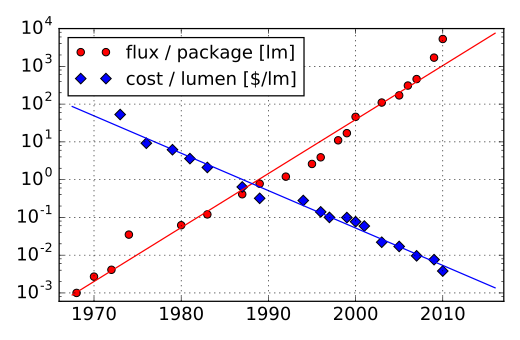
\includegraphics[width=0.5\textwidth]{figuras/haitz.png}
    \end{center}
    \caption{Ilustração da lei de Haitz, com quantidade de luz por LED em vermelho e custo por lúmen em azul.}
    \label{fig:haitz}
\end{figure}

A eficiência elevada e longa vida útil são fatores que vêm impulsionando investimentos nessa área. Uma linha de crédito, com duração de 5 anos, foi aprovada pelo BNDES \cite{bndes2} para fontes luminosas de alta potência em vista da rentabilidade segura que reside na substituição de fontes luminosas convencionais por aquelas que usam LEDs. Buscando incentivar o cenário da microelêtronica no Brasil, o credenciamento exige que as luminárias financiadas pelo BNDES empreguem circuitos de fabricação brasileira.

Outra importante vantagem dos LEDs é a sua capacidade de ter sua intensidade facilmente ajustada pela "dimmerização", isto é, rápido chaveamento de sua alimentação. Isto permite o controle rápido e fácil da intensidade luminosa permitindo um uso ainda mais eficiente.

\section{Objetivo}

O objetivo deste trabalho é projetar e implementar um sistema de iluminação com LEDs controlado pela internet por um aplicativo móvel ou página \textit{web}. Esse sistema deve ter as funcionalidades de ser ligado e desligado, ter sua intensidade ajustada manualmente pela internet e ainda ter um controle automático de intensidade. O sistema de iluminação conta com uma fita de LEDs, um sensor de luminosidade e um microcontrolador com comunicação WiFi para controlar o sistema. O protocolo de troca de mensagens é o MQTT que permite que o aplicativo e a página \textit{web} troquem mensagens com o sistema embarcado sobre a rede TCP/IP. O ajuste automático deve ser feito por um controle de malha fechada PID.

\section{Estrutura do Texto}

Este trabalho está organizado em capítulos nos quais o projeto é introduzido por motivações e objetivos, em seguida é dado um contexto de temas e conceitos, o desenvolvimento do projeto é descrito, testado e por fim são mostradas algumas conclusões sobre o projeto.

O Capítulo 2 apresenta os conceitos tratados no projeto e apresenta os temas abordados de forma clara e direta.

O Capítulo 3 descreve as funcionalidades do projetos que guiaram a escolha dos materiais usados e dos métodos empregados.

O Capítulo 4 demonstra, por meio de testes, as capacidades do sistema desenvolvido.

O Capítulo 5 apresenta as conclusões, experiências e sugestões para trabalhos futuros.
\chapter{Referencial Teórico}

\section{Iluminação de LED}

\subsection{LED}

O \acf{LED} mudou a forma como a humanidade gera luz. Atualmente são usados em inúmeras aplicações indicativas, iluminação, TVs e vários outros usos. O processo de emissão de luz por um material de estado-sólido estimulado por uma fonte de energia elétrica, denominado de eletroluminescência, foi primeiramente observado em 1907 por Henry Joseph Round (1881-1966) \cite{led}, quando investigava o uso de cristais de carbeto de silício (SiC conhecido também como \textit{corborundum}) como "cristais retificadores" responsáveis por demodular sinais modulados em amplitude nos rádios da época. A junção responsável pelo contato destes cristais e alguns metais (junção característica de diodos \textit{Schottky}) vinha sendo testada como possível substituta aos caros e ineficientes tubos de vácuo eletrônicos (ou válvulas termiônicas). Henry observou que alguns pontos do cristais brilhavam ao aplicar-se potenciais, na faixa de 10 a 110 V, com os contatos metálicos.

As primeiras investigações detalhadas sobre eletroluminescência foram feitas pelo inventor russo Oleg Vladimirovich Losev (1903-1942) que publicou seu primeiro artigo aos 20 anos em 1923, ainda sem educação formal, e reportou observar luz verde ao polarizar reversamente um retificador de junção metal-cristal de SiC. Losev também observou corretamente que a razão do fenômeno não tinha relação com incandescência pois ocorria a temperatura ambiente. Mais tarde, em 1933, Losev também estudou o efeito da eletroluminescência em junções semicondutoras "p-n" com destaque para suas observações quanto à relação entre a energia emitida pelo diodo e a energia de "\textit{gap}" do material.

Eletroluminescência é definida como a emissão de luz por um material semicondutor quando exposto a um campo elétrico. Um junção P-N, quando polarizada diretamente, conduz corrente elétrica pois ocorre um fluxo de elétrons da região de semicondutor tipo N para a região tipo P e consequentemente, um fluxo de "buracos", portadores fictícios de carga positiva, no sentido oposto. Os elétrons e buracos se recombinam e neste processo energia é liberada, pois os primeiros se encontram na camada de condução no semicondutor tipo N e os buracos, na camada de valência do semicondutor tipo P.

\begin{figure}[ht]
    \begin{center}
    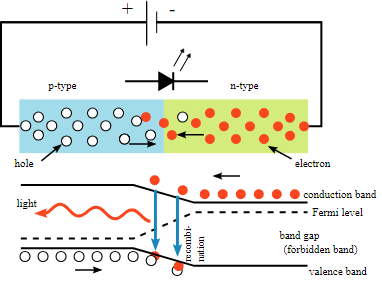
\includegraphics{figuras/led.PNG}
    \end{center}
    \caption[Diagrama de funcionamento do LED.]{Diagrama de funcionamento do LED. Acima, o esquema da junção p-n com o estímulo elétrico e abaixo o diagrama de banda de energia do semicondutor}
    \label{led}
\end{figure}

%By User:S-kei - File:PnJunction-LED-E.PNG, CC BY-SA 2.5, https://commons.wikimedia.org/w/index.php?curid=14985902 

A recombinação dos pares elétron-buraco libera energia pelo fato dos elétrons passarem para um nível menos energético \cite{rezende}. Uma vasta gama de materiais semicondutores apresenta uma estrutura de bandas de energia chamada de banda de "gap" indireto, e isso significa em resumo que a transição de elétrons entre os níveis energéticos não envolve apenas emissão ou absorção de luz (fótons), envolve também energia vibratória que gera calor (fônons). Alguns outros materiais têm o que se chama de banda de "gap" direta e a emissão de luz no caso desse tipo de material é bem mais eficiente que nos materiais de "gap" indireto. O comprimento de onda dos fótons emitidos está relacionado com energia de "gap" de forma que LEDs de diferentes materiais semicondutores emitem luz de cores distintas desde o infra-vermelho próximo até o ultra-violeta próximo. A famosa equação de \textit{Plank} demonstra a relação


    $$  E_g = h.v $$
    $$  v = \frac{c}{\lambda} $$
    $$  E_g = \frac{h.c}{\lambda} .$$
    
Onde "h" é a constante de \textit{Plank} e "c" é a velocidade da luz. A energia de "gap" e o comprimento de onda são, como visto, inversamente proporcionais e temos que para o extremo vermelho do espectro visível com comprimento de onda de 700nm requer um material com energia de "gap" de 1.77eV enquanto a energia necessária para obter o violeta extremo, em 400nm, é de 3.1eV. Abaixo vemos um quadro com as energias de "gap" e comprimento de onda característicos de alguns materiais semicondutores.

\begin{figure}[ht]
    \begin{center}
    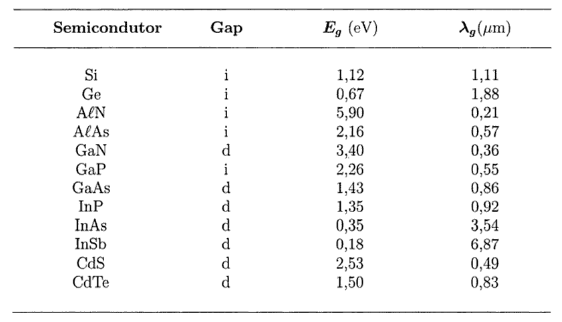
\includegraphics{figuras/semic.PNG}
    \end{center}
    \caption[Quadro de energias de gap e comprimentos de onda]{Quadro com os principais materiais semicondutores, tipo de banda, energia de gap e comprimento de onda resultante}
    \label{semicon}
\end{figure}

\subsection{Ergonomia da Iluminação}

A ergonomia é o estudo científico das relações homem e máquina no ambiente de trabalho, visando segurança e eficiência na interação entre estes. A norma regulamentadora que trata de ergonomia, a NR 17 \cite{norma}, traz orientações sobre luminosidade no ambiente de trabalho com o objetivo de proteger a saúde física e psicológica do trabalhador. Algumas das orientações da norma regulamentadora:

\begin{labeling}{17.5.3.3}
    \item[17.5.3] Em todos os locais de trabalho deve haver iluminação adequada, natural ou artificial, geral ou suplementar, apropriada à natureza da atividade.
    \item[17.5.3.1]  A iluminação geral deve ser uniformemente distribuída e difusa.
    \item[17.5.3.2] A iluminação geral ou suplementar deve ser projetada e instalada de forma a evitar ofuscamento, reflexos incômodos, sombras e contrastes excessivos.
    \item[17.5.3.3] Os níveis mínimos de iluminamento a serem observados nos locais de trabalho são os valores de iluminâncias estabelecidos na NBR 5413, norma brasileira registrada no INMETRO.
\end{labeling}

A NBR ISO/CIE 8995-1 \cite{normabr} substituiu a NBR 5413 e especifica condições de iluminação para ambientes de trabalho internos e visa a eficiência na execução de tarefas visuais com eficiência, conforto e segurança durante todo o tempo de trabalho, seja esta iluminação natural, artificial ou uma combinação de ambas. A fim de atingir esse objetivo vários critérios são levados em conta, entre eles estão: aspectos da cor da luz, cintilação e iluminância.

Esta legislação estabelece os valores de iluminâncias médias mínimas em serviço para iluminação artificial em interiores, onde se realizem atividades de comércio, indústria, ensino, esporte e outras. Estes valores estão condicionados a função do trabalhador e tempo de determinada tarefa. A iluminância é uma grandeza de luminosidade representada pela letra E, sua unidade de medida é o “lux”, para medí-la utiliza-se o luxímetro, e é definida como  "limite da razão do fluxo luminoso recebido pela superfície em torno de um ponto considerado, para a área da superfície quando esta tende para o zero." (NBR 8995-1, 2013).  A iluminância pode impactar em como uma pessoa percebe e realiza uma tarefa visual, de forma que altos valores de iluminância causam desconforto e ofuscamento e baixos valores tornam o ambiente de trabalho sem estímulo e tedioso.

%A cintilação e efeitos estroboscópicos são causado pelo chaveamento frequente ou oscilação da iluminância em função de aspectos elétricos da iluminação e pode provocar distração e efeitos fisiológicos como dores de cabeça. Podem ainda levar a situações de risco pela alteração da percepção de máquinas de rotação sincronizadas com a frequência de oscilação da iluminância. Este efeito é análogo ao de ver, em filmagens, a roda de um carro em movimento que parece estar girando devagar ou estar parada; o mesmo pode acontecer em uma fábrica com uma máquina síncrona iluminada por uma fonte de luz alimentada pela mesma rede elétrica que alimenta a máquina.%

\section{Internet das Coisas}

Ao longo da história, vários pensadores, cientistas e inventores fizeram previsões convergentes para o futuro, previsões de que um dia o mundo teria uma rede interconectada de computadores e sensores. Hoje vemos essas previsões tomarem forma e podemos vislumbrar esse futuro imaginado por grandes mentes do passado. Nikolas Tesla disse certa vez em uma entrevista em 1926: “... o planeta inteiro se tornará um cérebro gigante, o que significa que todas as coisas serão partes reais e harmônicas de um todo… e os instrumentos que nos permitirão realizar isso serão incrivelmente mais simples que os telefones atuais. Qualquer homem será capaz de carregar um seu próprio bolso”. Já o primeiro dispositivo cotidiano a se conectar a internet foi uma torradeira criada por John Romkey em 1990 e que se conectava a um computador pela pilha de protocolos TCP/IP (\acl{TCP} / \acl{IP}) podendo ser ligada ou desligada pela internet.

Tecnologias correlatas a \ac{IoT} vêm sendo adotadas, nos últimos anos, por empresas de todos os portes e abrindo espaço para novos empreendimentos. Não há restrições claras para os limites de aplicações para \ac{IoT}; aliada a outra importante tecnologia que vem sendo extensivamente explorada, a inteligência artificial, a \ac{IoT} consegue prover vantagens como aumento de produtividade, extrema versatilidade na obtenção de dados e redução de despesas. Um exemplo interessante é a aplicação de dispositivos conectados à rede na produção do leite \cite{milk} na qual produtores têm colocado sensores nos calcanhares, pescoço, mamas e intestino das vacas para prever com exatidão os ciclos férteis dos animais, medir a qualidade do leite antes de extraí-lo e monitorar a saúde da vaca.

\begin{figure}[ht]
    \begin{center}
    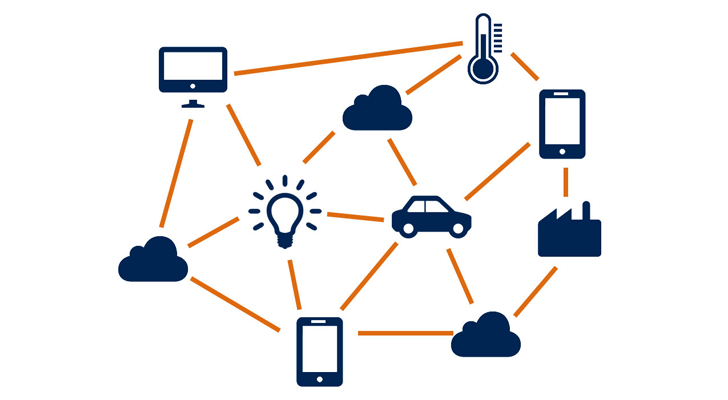
\includegraphics[width=0.7\textwidth]{figuras/iot}
    \end{center}
    \caption[Esquema dos elementos da Internet das Coisas.]{Esquema dos elementos da Internet das Coisas.}
    \label{iot}
\end{figure}

O mercado de \ac{IoT} pode ser separado em aplicações de consumo, da indústria e de serviços de infraestrutura da própria internet das coisas. O ramo voltado ao consumidor amplo é caracterizado principalmente por aplicações domiciliares como sistemas de segurança conectados e automação residencial, além de dispositivos vestíveis como monitores de sinais biológicos e relógios “inteligentes”. O setor industrial faz uso da internet das coisas em soluções de logística, agropecuária, sensoriamento em geral, planejamento urbano, monitoramento da rede elétrica, e vários outros exemplos. Para possibilitar que todos esse serviços de \ac{IoT} funcionem, há várias plataformas de infraestrutura de rede, sistemas embarcados, plataformas de software e serviços de armazenamento e análise de dados. Gigantes da tecnologia como “\textit{Google}”, “\textit{Microsoft}” e “\textit{Amazon}” têm setores totalmente voltado para \ac{IoT} e serviço de nuvem como o “\textit{Google Cloud}”, o “\textit{Microsoft Azure}” e o “\textit{Amazon Web Services}”.

\subsection{Redes de Computadores}

A comunhão dos computadores e das comunicações foi uma das principais revoluções tecnológicas modernas dando origem ao campo de redes de computadores com a demanda de organizar a comunicação entre computadores e criar sistemas computacionais para fazer essa comunicação.

Diz-se que uma rede de computadores é definida por dois ou mais computadores que, interligados por um meio físico, são capazes de trocar dados \cite{redes}. O conceito não especifica qual o meio físico que interliga os computadores que pode ser cabos metálicos, fibras óticas, micro-ondas, ondas de infravermelho; mas limita o meio a apenas um tipo, de forma que a “ampla rede mundial” (\textit{World Wide Web}) não é uma rede mas uma “rede de redes” e que a internet não é uma rede, e sim um sistema distribuído que, apesar de ser composto por vários computadores, é um sistema de softwares que opera sobre a rede e que dá a impressão ao usuário de ser um sistema coerente, uma rede não apresenta essa coerência aparente.

A \textit{World Wide Web} funciona de acordo com o modelo de cliente/servidor no qual um serviço cliente interage na rede por solicitações ao serviço servidor que responde a essas solicitações, podemos dizer também que o servidor provê recursos que os clientes consomem.

\subsection{A tecnologia \ac{WiFi}}

A popularização de computadores pessoais portáteis (notebooks) trouxe consigo a demanda que o acesso à internet se tornasse, também, móvel e assim foram desenvolvidas algumas arquiteturas de rede baseadas em ondas eletromagnéticas. A existência de diversos tipos de conexão sem fio (wireless) evidenciou a necessidade de uma padronização e assim o \ac{IEEE} lançou o padrão “802.11” para redes locais \cite{wifi} com uma série de especificação de controle de acesso ao meio (MAC) e camada física nas frequências de 900 MHz, 2.4, 3.6, 5 e 60 GHz com larguras de banda mais usuais de 20 ou 22 MHz e taxas de 1 até 3500 MB/s. Diversas revisões subsequentes do padrão como “a”, “b”, “g”, “n” especificam frequência, largura de banda, modulação entre outros fatores; a maioria dos dispositivos com internet sem fio é versátil para trabalhar com múltiplos modelos do padrão.

A \acf{WiFi} é uma marca da Wi-Fi Alliance, organização que promove a tecnologia e certifica produtos que obedecem a alguns requisitos de interoperabilidade do padrão \ac{IEEE} 802.11. Inicialmente, a variante do padrão 802.11 adotada pelo WiFi foi o "b" com taxas de transferência de até 11 MB/s, atualmente o padrão "g" vinha sendo usado e o padrão "n" começou a ser suportado desde 2009, com taxas de transferência de até 100 MB/s, todos estes operando na frequência de 2.4 GHz. A grande maioria dos roteadores WiFi comercializados hoje em dia suportam o padrão "802.11 b/g/n" com suporte às frequências de 2.4 e 5 GHz 

\section{\ac{MQTT}}

O \acf{MQTT} é um protocolo baseado em publicações e subscrições (ou assinaturas) de conectividade em rede para M2M (\textit{Machine to machine}) e \ac{IoT} construído sobre a camada subjacente de internet \ac{TCP}/\ac{IP}. Ele foi criado com o intuito de ser leve, simples e de fácil aplicação com o objetivo de conectar sensores em dutos de petróleo a satélites. A primeira versão do protocolo foi apresentada em 1999 por Andy Stanford-Clark da IBM e Arlen Nipper, e no final de 2014 se tornou um padrão aberto OASIS \cite{oasis} com suporte para diversas linguagens de programação.

O MQTT é um protocolo de transporte de mensagens com comunicação assíncrona o que torna possível desacoplar os usuários do sistema no espaço e no tempo, e viabiliza seu uso em situações com redes que não são confiáveis. Não obstante o protocolo apresenta codificação simples e quantidade mínima de dados de cabeçalho (informações além dos dados que se deseja transportar) em seus pacotes, características que implicam em uma alta eficiência de banda.

Como este protocolo funciona com o paradigma de publicações/subscrições para troca de mensagens entre as partes, ou clientes, e para isso ele apresenta um elemento mediador ao qual é dado nome \textit{broker}. Clientes que desejam enviar mensagens devem publicá-las em tópicos e clientes que querem receber mensagens de outros clientes devem subscrever os tópicos. O \textit{broker} tem o papel de conectar os clientes e mediar a troca de mensagens em tópicos. Em um sistema qualquer cliente pode subscrever qualquer tópico e publicar em qualquer tópico.

A estrutura do MQTT permite que os clientes sejam independentes no espaço, isto é, um cliente não precisa saber o endereço (IP ou porta) de outro para enviá-lo alguma mensagem; e torna-os independentes no tempo permitindo que o “ouvinte” não precise estar ativo quando alguma mensagem for enviada a ele.

\subsection{\textit{Broker} e Clientes}

Os elementos de uma rede baseada em MQTT baseada são, comumente, os clientes e um \textit{broker}. O broker funciona como um servidor que recebe as mensagens publicadas, classificadas por tópicos, e as encaminha para os clientes subscritos nos tópicos determinados. Clientes, por sua vez, são qualquer elemento que publique ou receba mensagens por subscrição podendo ser desde um sensor ou um atuador conectado, uma aplicação web que processa os dados, ou ainda um aplicativo móvel com poder de observar o comportamento dos sensores e publicar ações para os atuadores.

\subsection{Publicações e Subscrições}

O paradigma de comunicação por publicações e subscrições (ou simplesmente “\textit{PubSub}”) é um paradigma no qual remetentes, chamados de publicadores, não especificam quais serão os destinatários, chamados de subscritores, das mensagens enviadas; em vez disso as mensagens são classificadas por assuntos, chamados de tópicos, assim um cliente que publica uma mensagem não controla quais clientes a receberam ou, ainda, se será recebida por qualquer cliente. Consequentemente, clientes que subscrevem determinados tópicos não, necessariamente, sabem qual cliente originou determinada mensagem apesar de tópicos estarem comumente atrelados a publicadores, isso significa que comumente um tópico têm mensagens publicadas por um único publicador.

Tópicos são representados por “\textit{strings}” organizadas de forma hierárquica por níveis os quais são separados por barras (“/”) lembrando o padrão URI de endereços. Os tópicos permitem filtrar mensagens por categorias, clientes ou tipo de dados. Isto significa que o sistema de automação de uma casa com vários sensores de temperatura e umidade pode ter alguns de seus tópicos nomeados da seguinte forma:

\begin{center}
    \texttt{“home/jardim/sensor1/temperatura”}
    
    \texttt{“home/jardim/sensor3/umidade”}
\end{center}

O sistema de tópicos apresenta ainda flexibilidade no que diz respeito ao acesso generalizado a mensagens. Usando o exemplo anterior, caso um cliente deseje subscrever todos os tópicos referentes a temperatura, ele pode usar caracteres “coringa” como “+” ou “\#” da seguinte forma:

\begin{center}
    \texttt{“home/+/+/temperatura”}
    
    \texttt{“home/\#/\#/temperatura”}
\end{center}

\begin{figure}[ht]
    \begin{center}
    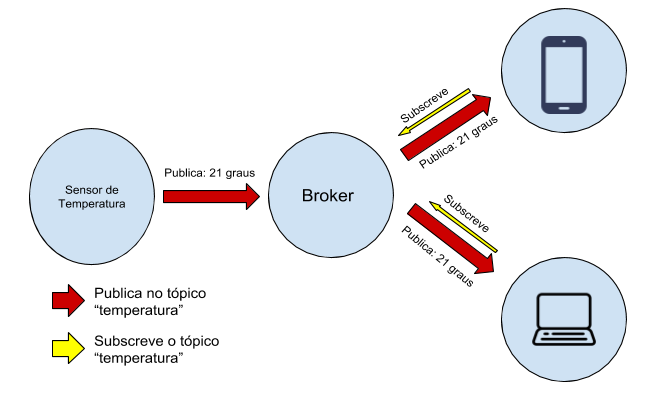
\includegraphics[width=0.7\textwidth]{figuras/mqtt.PNG}
    \end{center}
    \caption[Ilustração do funcionamento do protocolo MQTT.]{Ilustração do funcionamento do protocolo MQTT com três clientes e o broker trocando mensagens pelo tópico "temperatura".}
    \label{mqtt}
\end{figure}

A troca de mensagens funciona da seguinte forma:
\begin{itemize}
    \item[1 -] O cliente conecta-se ao \textit{broker} por meio de uma conexão TCP/IP e pode assinar (ou subscrever) qualquer tópico de mensagens do \textit{broker}.
    \item[2 -] O cliente pode publicar mensagens ao enviar o tópico e o conteúdo da mensagem (também chamado de \textit{payload}) ao \textit{broker}.
    \item[3 -] O broker encaminha as mensagens publicadas aos clientes.
\end{itemize}

\subsection{QoS}

Qualidade de serviço (\acl{QoS}) é uma padronização das capacidades de troca de dados em uma rede que determina fatores como a previsibilidade, retardo e a qualidade geral da comunicação; mais especificamente no caso do protocolo MQTT, os níveis de qualidade de serviço (0, 1 e 2) são uma espécie de “acordo” entre o transmissor e o receptor da mensagem quanto a garantia de entrega de uma mensagem, e isso impacta diretamente a previsibilidade da comunicação.

Os três níveis de QoS no MQTT são:
\begin{itemize}
    \item[0 -] Não há garantia de entrega.
    \item[1 -] Mensagem é entregue pelo menos uma vez (pode ser mais).
    \item[2 -] A mensagem é entregue exatamente uma vez.
\end{itemize}

A garantia de entrega dos níveis 1 e 2 é devido a confirmações de recebimento e reenvio em caso de falha. O nível 0 não inclui confirmações de entrega ou reenvios, é comumente chamado de nível de melhor esforço possível ou “\textit{fire and forget}” (atire e esqueça); apesar de ser o nível de pior previsibilidade, apresenta também a menor latência de comunicação.

Ao usar o nível de QoS 1, um cliente que envia uma mensagem ao broker, ou o inverso, contará com a garantia que essa mensagem será entregue pelo menos uma vez, mas pode ser mais de uma vez. Uma mensagem publicada pelo cliente será armazenada por ele até que receba uma confirmação, um “\textit{puback}” (confirmação de publicação), com a mesma identificação da mensagem enviada. Caso não receba a confirmação até determinado tempo (“\textit{ack timeout}”) a mensagem será reenviada com, com informação que está duplicada, periodicamente até o recebimento do “\textit{puback}”.

O nível mais alto de QoS, 2, é o que provê mais previsibilidade e envolve a maior quantidade de troca de informações na troca de uma mensagem. Esse nível apresenta confirmação de recebimento e confirmação de recebimento da confirmação. A maioria de serviços de MQTT baratos ou grátis, para testes e "hobbistas", não dão suporte ao QoS de nível 2.

\section{Sistemas Embarcados}

Uma definição sucinta de sistema é um conjunto de processos ou mesmo sistemas conectados que realizam uma ou mais tarefas como um todo. Como o nome sugere um sistema embarcado é um sistema eletrônico que faz parte de um sistema maior com a função de, muitas vezes, controlar, interfacear, observar outros sistemas eletrônicos ou não. É um programa computacional, ou \textit{software}, que é executado por um sistema físico, o \textit{hardware}, de capacidades adequadas ou projetadas para a tarefa a ser executada, diferente de computadores pessoais, de propósito geral, que possuem capacidade de executar uma grande variedade de tarefas à demanda do usuário.

Os sistemas embarcados são parte de fundamental da maioria dos sistemas eletrônicos usados atualmente por apresentar padronização de comunicação entre estas unidades, facilidade e simplicidade de processamento de sinais e consumo de energia otimizado. Uma característica importante de sistemas embarcados é que existem arquiteturas dos mais variados tipos, que são especificados para executar os mais variados tipos de tarefas: desde arquiteturas que suportam sistemas operacionais complexos para processamento de imagens em tempo real, até arquiteturas simples com poucos transistores e outros componentes que realizam tarefas como ligar uma lâmpada ou contar tempo.

\subsection{Microcontroladores}

Microcontroladores são sistemas embarcados cuja função é a de controlar o sistema do qual fazem parte. Dentro da classe de sistemas dedicados estão os microcontroladores que são compostos, em geral, por uma unidade central de processamento (CPU), memória não-volátil para dados e instruções, memória volátil de acesso aleatório (RAM), oscilador e periféricos que geram entradas ou recebem saídas do processador como contadores, \textit{timers}, módulos de comunicação seriais e paralelos, conversores analógicos e digitais . Microcontroladores estão presentes em quase todos equipamentos eletrônicos que se possa imaginar: a indústria de eletrônica de consumo e a indústria automobilística fazem uso extensivo de microcontroladores.

\begin{figure}[ht]
    \begin{center}
    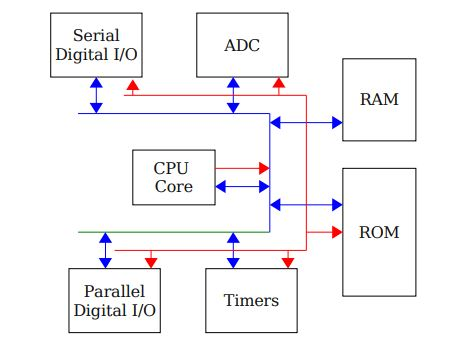
\includegraphics[width=0.4\textwidth]{figuras/micro.JPG}
    \end{center}
    \caption[Diagrama de blocos de um microcontrolador.]{Diagrama de blocos de um microcontrolador com o núcleo de processamento e seus diversos periféricos}
    \label{micro}
\end{figure}

\subsection{ESP-8266}

O ESP-8266 \cite{esp} é um \acf{SoC} com capacidade de comunicação \ac{WiFi} padrão 802.11 b/g/n da fabricante chinesa \textit{Espressif}. Conta com uma CPU de 32 bits RISC (\textit{Reduced Instronction Set Computer}), o \textit{Xtensa} LX106 da \textit{Cadence Tensilica} de baixa potência (menos de 1 mW em \textit{standby}), possui \textit{clock} de 80 MHz, uma ROM de \textit{boot} de 64KB, uma RAM de instruções de 64 KB e uma RAM para dados de 96 KB. Possui a pilha TCP/IP já integrada. Sua tensão de alimentação recomendada é de 3.3V.

\begin{figure}[ht]
    \begin{center}
    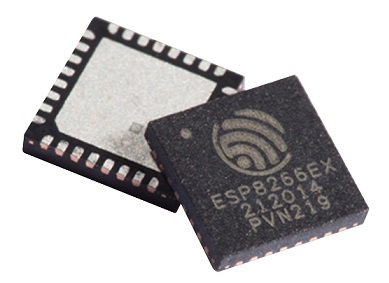
\includegraphics[width=0.3\textwidth]{figuras/esp8266.jpg}
    \end{center}
    \caption[ESP-8266 em seu encapsulamento QFN.]{Ilustração do circuito integrado ESP-8266 em seu encapsulamento QFN.}
    \label{esp8266}
\end{figure}

O ESP8266 possui interfaces "UART", "I2C" (apenas a função de mestre implementada em suas bibliotecas de desenvolvimento de \textit{software} oficial, mas há implementações para escravo I2C da comunidade), "SPI" (com três pinos de \textit{device enable} além dos outros pinos usuais do protocolo). Possui 16 pinos de uso geral podendo ser configurados com pull-up/down internos, interrupção por nível ou borda em seus pinos de entrada e saída, opção configurável de saída open-drain ou push-pull, ou ainda saída analógica de PWM com resolução de 10 bits em qualquer pino e uma entrada analógica (ADC). Seus pinos possuem proteção contra sobrevoltagem de até 5,8 V e conseguem fornecer até 12 mA de corrente cada um.

\begin{figure}[ht]
    \begin{center}
    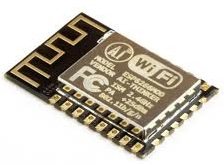
\includegraphics[width=0.3\textwidth]{figuras/esp12.jpg}
    \end{center}
    \caption[Kit de desenvolvimento ESP-12.]{Ilustração kit de desenvolvimento ESP-12 baseado no ESP-8266}
    \label{esp12}
\end{figure}

A \textit{Espressif} comercializa diferentes módulos baseados no ESP8266, numerados de 1 até 12, que facilitam o desenvolvimento e a produção de produtos por já integrar circuitos ou chips de antena, sistema de alimentação e outros circuitos com o seu SoC. O ESP-01, por exemplo, possui apenas oito pinos, sendo dois deles "VCC" e "GND", e foi desenvolvido para ser usado como um simples modulo WiFi-serial. O ESP-12F possui os 16 GPIOs disponíveis e uma memória flash externa de 4MB "SPI". Esse módulo é usado na maioria das plataformas de desenvolvimento do ESP-8266, como o “\textit{NodeMCU}” e o “\textit{Wemos D1 Mini}”. Estas plataformas possuem recursos que facilitam o desenvolvimento como interface USB-serial, botão de \textit{reset} e conectores apropriados para \textit{protoboards}.

\chapter{Materiais e Ferramentas}

A descrição dos elementos físicos usados no projeto da lâmpada inteligente pode ser resumida pelo esquema geral do projeto na Figura \ref{esquema}.

\begin{figure}[ht]
    \begin{center}
    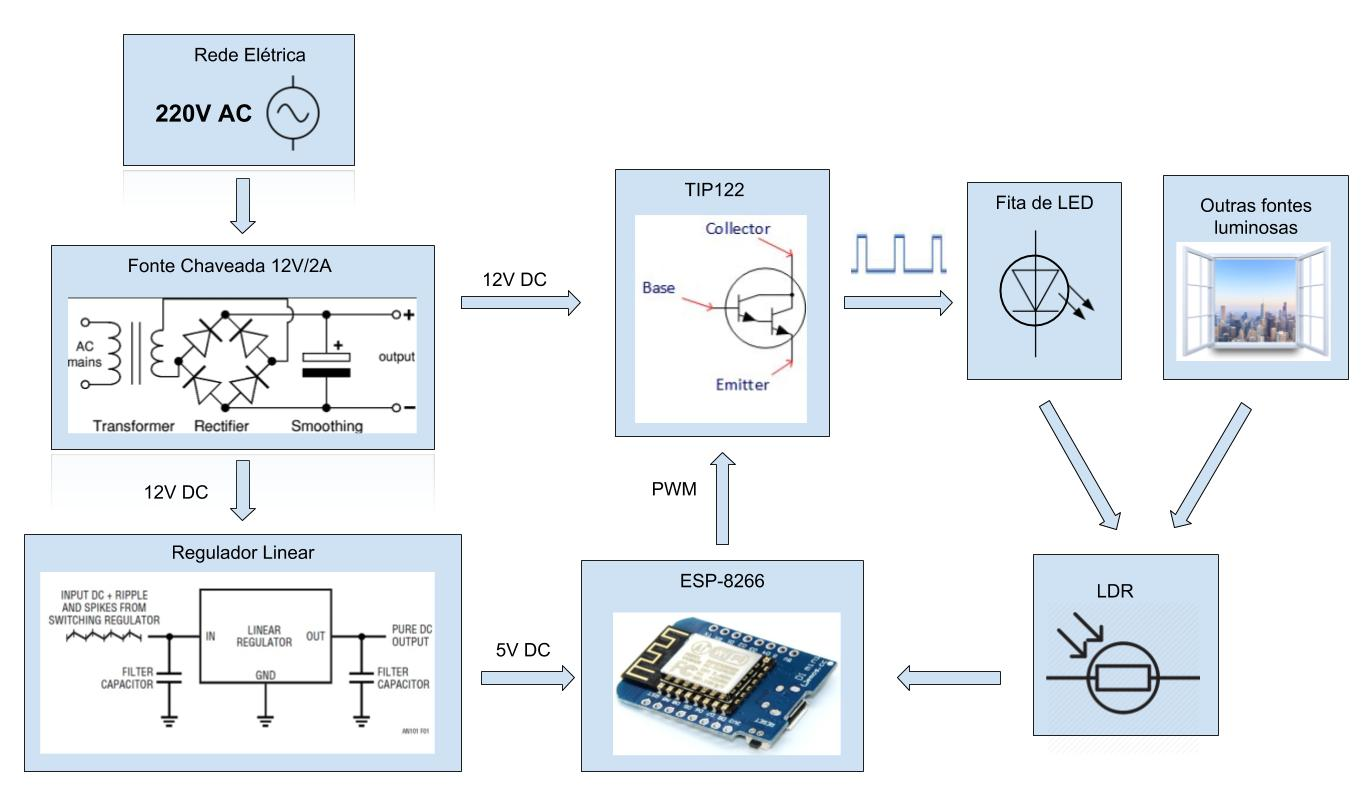
\includegraphics[width=\textwidth]{figuras/esquema_eletrico.jpg}
    \end{center}
    \caption[Esquema geral do projeto da fita de LED MQTT.]{Ilustração do funcionamento do protocolo MQTT com três clientes e o broker trocando mensagens pelo tópico "temperatura".}
    \label{esquema}
\end{figure}

\section{Alimentação}

A fonte de alimentação elétrica do projeto é uma fonte comercial de 12V/1A de padrão comercial “\textit{bivolt}” com plugue P4. Os 12V fornecidos pela fonte serão partilhados pela fonte de iluminação e pelo sistema embarcado. Um regulador baseado no CI AMS1117 será usado para transformar os 12V da fonte em 5V para alimentar o sistema com o microcontrolador. Esse regulador têm sua tensão de saída fixa em 5V e apresenta algumas funcionalidades como limitador interno de corrente e auto-desligamento térmico, e com o arrefecimento adequado ele pode fornecer até 1A que já é mais que o suficiente para o ESP-8266 que consome em torno de 220 mA durante curtos períodos quando está transmitindo via WiFi.

\begin{figure}[ht]
    \begin{center}
    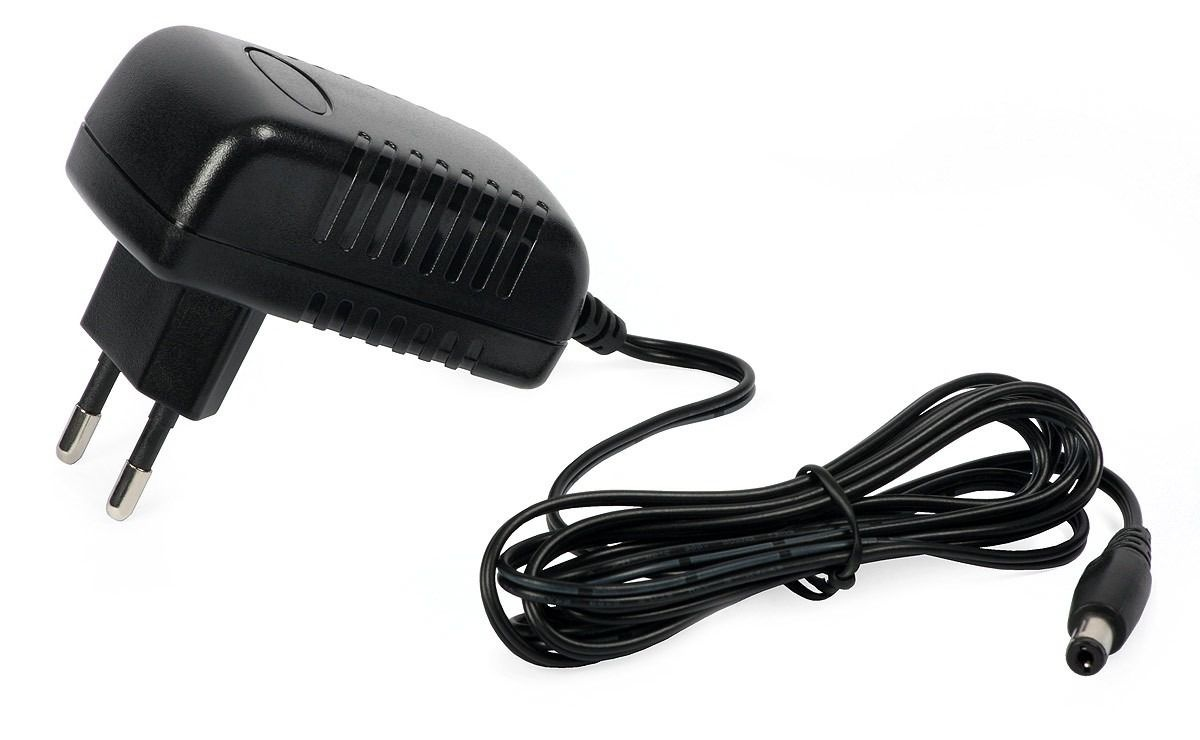
\includegraphics[width=0.5\textwidth]{figuras/fonte.jpg}
    \end{center}
    \caption[Ilustração da fonte chaveada de 12V.]{Ilustração da fonte chaveada de 12V com capacidade de fornecer até 2A.}
    \label{fonte}
\end{figure}

\section{Módulo Microcontrolador}

Como mencionado, o microcontrolador escolhido para o projeto é o ESP-8266 que inclui capacidade de comunicação WiFi. A própria fabricante do CI comercializa alguns módulos que facilitam o desenvolvimento com o ESP-8266 com antenas, LED, memória \textit{flash} e outros periféricos. Um desses módulos, o ESP-12 é usado por diversas empresas para fabricarem seus kits de desenvolvimento com ainda mais facilidades para o desenvolvedor. O kit usado neste projeto é “\textit{Wemos D1 Mini}” que conta com conversor USB-serial, regulador de tensão para transformar os 5V DC provenientes da porta "USB" ou da alimentação externa para os 3.3V DC que o ESP-8266 demanda, oscilador, botão para \textit{reset} e conectores para os pinos de entrada e saída.

\begin{table}
    \centering
    \label{wemos_dados}
    \caption{Especificações do kit \textit{Wemos D1 Mini}}
    \begin{tabular}{ll} 
        \hline
        Kit de desenvolvimento          & Wemos D1 Mini  \\ 
        \hline
        SoC                             & ESP-8266       \\ 
        \hline
        Pinos de I/O digitais           & 11             \\ 
        \hline
        Entradas analógicas             & 1 (3,2V máx)   \\ 
        \hline
        Clock                           & 80 MHz         \\ 
        \hline
        Memória \textit{flash}          & 4 MB           \\
        \hline
    \end{tabular}
\end{table}

O pino de entrada analógica do módulo usado tem uma tensão máxima especificada de 3,2V, apesar de a tensão máxima de entrada do ESP-8266 ser de 1V segundo suas características elétricas \cite{esp}. Isto se deve ao fato de o módulo "\textit{Wemos D1 Mini}" apresentar um divisor de tensão conectado ao pino de entrada analógica do SoC fazendo com que a tensão aplicada a este pino seja mapeada de um intervalo de, 0 a 3,2V no devido pino do módulo, para um intervalo de 0 a 1V no pino do ESP-8266.

\begin{figure}[ht]
    \begin{center}
    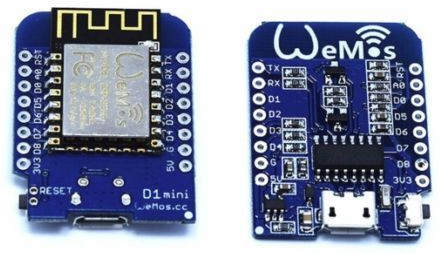
\includegraphics[width=0.4\textwidth]{figuras/wemos.PNG}
    \end{center}
    \caption[Ilustração do módulo \textit{Wemos D1 Mini}.]{Módulo \textit{Wemos D1 Mini} baseado no ESP-8266 visto de cima e de baixo.}
    \label{wemos}
\end{figure}

\section{Sensor de Luminosidade}

O sensor de luminosidade é um "fotoresistor" ou \acf{LDR} cuja resistência, geralmente, diminui com o aumento da intensidade luminosa linearmente. Geralmente são materiais semicondutores de alta resistividade, mas que quando expostos à luz, têm elétrons liberados em sua camada de condução aumentando assim sua condutividade por isso são geralmente chamados de células fotocondutivas. Existem LDRs sensíveis a faixas de radiação ultravioleta, infravermelho e a luz visível, que são os mais comuns.

O LDR usado \cite{ldr} é feito do material semicondutor CdS e apresenta uma curva de resistência em função da intensidade luminosa como mostrada na figura \ref{reta}. Os valores mostrados podem variar um pouco com a temperatura e existe um comportamento transiente quando a luminosidade é variada bruscamente de tempos da ordem de 100ms, o que não se torna relevante para medições menos frequentes que uma repetição por minuto, por exemplo.

\begin{figure}[htp]
    \begin{center}
    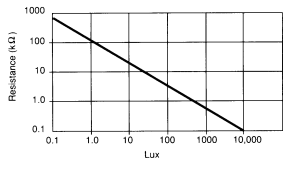
\includegraphics[width=0.4\textwidth]{figuras/reta.PNG}
    \end{center}
    \caption[Gráfico da reisitência \textit{versus} intensidade luminos do LDR.]{Gráfico da reisitência \textit{versus} intensidade luminos do LDR.}
    \label{reta}
\end{figure}

\section{Fita de LED}
A fonte de iluminação é uma fita de LED branca que consiste de elementos de três LEDs e um resistor em série para limitar a corrente, com vários desses elementos ligados em paralelo o que permite que todos os elementos sejam submetidos à mesma tensão e que a fita possa ser cortada em determinados pontos e continue funcionando. A fita de LED adquirida para o projeto tem as especificações listadas na Tabela 3.2.

\begin{figure}[htp]
    \begin{center}
    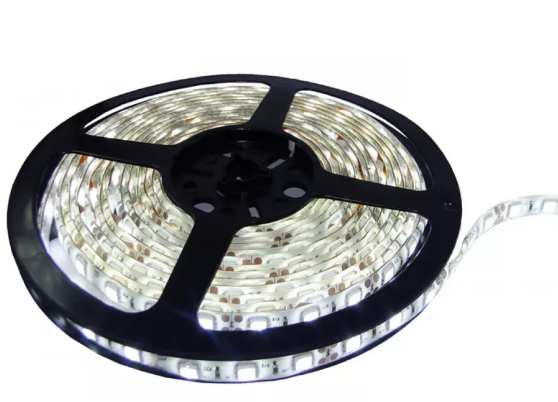
\includegraphics[width=0.3\textwidth]{figuras/fitaled.PNG}
    \end{center}
    \caption[Ilustração da fita de LED branca.]{Ilustração da fita de LED de cor branca fria de 12V.}
    \label{fitaled}
\end{figure}

 

\begin{table}
    \centering
    \label{fitaled_dados}
    \caption{Especificações da fita de LED branca}
    \begin{tabular}{ll} 
        \hline
        Tensão de Operação (V)  & 12            \\ 
        \hline
        Consumo por metro (W/m) & 4.8           \\ 
        \hline
        Comprimento (m)         & 5             \\ 
        \hline
        LEDs por metro          & 60            \\ 
        \hline
        Temperatura da cor (K)  & 6000(frio)    \\
        \hline
    \end{tabular}
\end{table}

O controle da luminosidade será feito por chaveamento da alimentação da fita de LED com \acf{PWM}, técnica que permite controlar digitalmente a potência entregue a atuadores ao determinar a parcela do período em nível lógico alto, de um sinal alternado. O microcontrolador irá chavear um transistor \textit{darlington} “TIP122” \cite{tip122}.

\section{Ferramentas de Desenvolvimento}

\subsection{\textit{Broker} MQTT}

O \textit{broker}, ou servidor, MQTT responsável pelo controle das mensagens intercambiadas na rede será o \textit{broker} da "\textit{Adafruit}" \cite{adafruit}. O serviço oferecido pela \textit{Adafruit} conta com um  \textit{broker} MQTT configurado com níveis de QoS 0 e 1, tópicos especiais como o "\texttt{time/seconds}" que fornece um número de segundos passados desde primeiro de janeiro de 1970 (\textit{Unix Time}) ou o tópico "\texttt{(username)/throttle}" que indica se a limitação de frequência de publicações foi atingida (que na versão grátis do serviço é de 60 vezes por minuto). O seviço da \textit{Adafruit} fornece também uma biblioteca da MQTT própria para \textit{Arduino} que define várias funções de \textit{callback} de subscrições e rotinas de conexão, desconexão e outras.

Uma interface de controle e visualização \textit{web} também é fornecida pela \textit{Adafruit} com possibilidade de implementação de botões, mostradores de valores, gráficos em tempo real, entre outras funcionalidades.

\subsection{Ambiente de Desenvolvimento de \textit{Software}}

O ESP-8266 possui um conjunto de bibliotecas e ferramentas, cujo objetivo é produzir código que, quando compilado, pode ser gravado na memória de programa e executado. Essas ferramentas levam o nome de "SDK" (\textit{Software Development Kit}) e são fornecidas, oficialmente, pela fabricante \textit{Espressif}. Uma comunidade de desenvolvedores do ESP-8266 criou uma estrutura de interfaces e adaptações (\textit{framework}) de código aberto para a SDK oficial para que fosse possível programar com a linguagem "C++" e usar as bibliotecas do \textit{Arduino}.

O desenvolvimento do software foi feito na IDE (\textit{Integrated Development Environment}) "\textit{Visual Studio Code}" da "\textit{Microsoft}" que é essencialmente um editor de texto de código aberto, muitas opções de customização e capacidade de conexão com extensões de terceiros. Uma dessas extensões foi usada, o "PlatformIO", Figura \ref{pio}, que é uma plataforma que conta com compiladores e outras ferramentas de diversos microcontroladores como \textit{Arduino}, ARM, \textit{Atmel} e vários outros. A extensão conta ainda com terminal virtual, monitor de porta serial, ferramentas de depuração de código e suporte à versionamento de código online.

\begin{figure}[ht]
    \begin{center}
    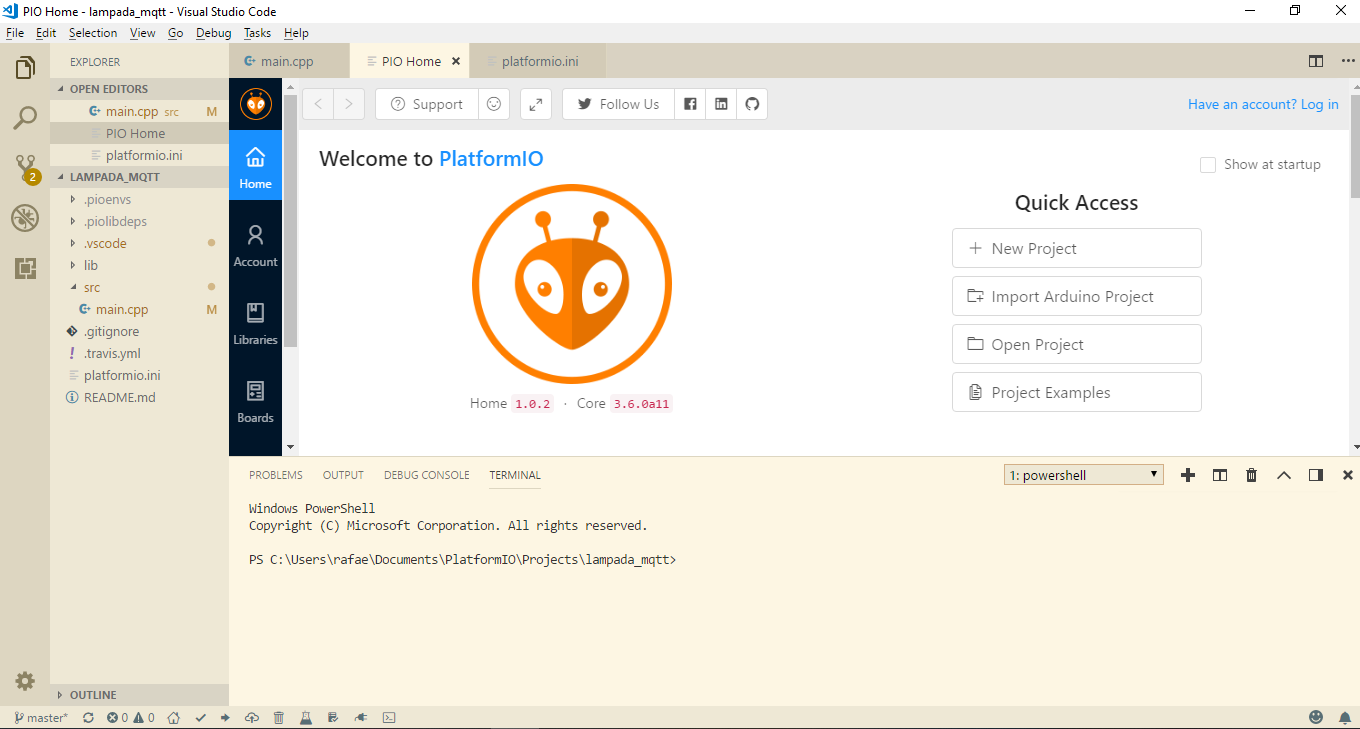
\includegraphics[width=\textwidth]{figuras/pio.PNG}
    \end{center}
    \caption[Ilustração do Visual Studio Code com o PlatformIO.]{Ilustração do ambiente de desenvolvimento "Visual Studio Code" com a extensão "PlatformIO".}
    \label{pio}
\end{figure}

\subsection{Bibliotecas}

Como mencionado, a programação foi feita na linguagem de programação "C++" com algumas bibliotecas de terceiros. A primeira a ser mencionada é a biblioteca do \textit{Arduino} que disponibiliza várias funções e definições que permitem uma grande simplicidade legibilidade do código escrito \cite{arduino}.

Outra biblioteca usada foi "Esp8266WiFi" \cite{espwifi}que disponibiliza várias rotinas relativas a conexão do ESP-8266 como a rede WiFi, reconexão, códigos relativos a camada TCP/IP e outros detalhes importantes para que o uso da internet com o microcontrolador seja possível.

A biblioteca "WiFi \textit{Manager}" \cite{wifimng} foi também usada e permitiu automatizar e generalizar o processo de autenticação do projeto para qualquer rede WiFi por meio da criação de uma página \textit{web} pela qual o usuário pode escolher a rede desejada e informar sua senha para que o ESP-8266 se conecte e salve essas informações em caso de reconexão.

\chapter{Desenvolvimento do Projeto}

O projeto do sistema de iluminação controlado pela internet foi desenvolvido com o objetivo de apresentar algumas funcionalidades, dadas as limitações, e demonstrar a potencialidade de economia de energia. As funcionalidades propostas foram as de, remotamente, ligar e desligar a iluminação; apresentar dois modos de controle da luminosidade: O modo manual no qual o usuário poderá escolher a intensidade da fita de LED e o modo automático no qual o sistema manterá um nível mínimo de luminosidade, caso as fontes de luz externas ao sistema apresentem intensidade menor que o nível escolhido pelo usuário para o modo automático. A demonstração da economia de energia do sistema é baseada na comparação das estimativas do consumo da iluminação com intensidade máxima e do consumo com intensidade controlada automaticamente.

\section{Montagem}

\section{Programação}

\section{Interfaces de Usuário}

\subsection{Aplicativo Móvel}

\subsection{Interface \textit{Web}}

\section{Teste Proposto}

%%
%% Parte pós-textual
%%
\backmatter

% Apêndices
% Comente se não houver apêndices
%\appendix

% É aconselhável criar cada apêndice em um arquivo à parte, digamos
% "apendice1.tex", "apendice.tex", ... "apendiceM.tex" e depois
% incluí-los com:
% \chapter{Código Fonte}

\lstset{
    frame=tb,
    language=C++,
    aboveskip=3mm,
    belowskip=3mm,
    showstringspaces=false,
    columns=flexible,
    basicstyle={\small\ttfamily},
    numbers=left,                    
    numbersep=5pt,                  
    numberstyle=\tiny\color{gray},
    keywordstyle=\color{blue},
    commentstyle=\color{dkgreen},
    stringstyle=\color{mauve},
    breaklines=true,
    breakatwhitespace=true,
    tabsize=4,
    captionpos=b
}

\begin{lstlisting}

/************************** Libraries ***************************/
#include <Arduino.h>
#include <ESP8266WiFi.h>
#include "Adafruit_MQTT.h"
#include "Adafruit_MQTT_Client.h"

// Includes do Wifi Manager
#include <DNSServer.h>
#include <ESP8266WebServer.h>
#include <WiFiManager.h>         //https://github.com/tzapu/WiFiManager

/********************* WiFi Access Point *************************/

#define WLAN_SSID       "GVT-4238"
#define WLAN_PASS       "6703003118"

/********************* Adafruit.io Setup *************************/

#define AIO_SERVER      "io.adafruit.com"
#define AIO_SERVERPORT  1883
#define AIO_USERNAME    "RafaelMQ"
#define AIO_KEY         "f6ed222e222c446088110578b7bd0146"

/********************* PIN DEFINITIONS **************************/
#define USER_LED D1

#define pwm_map_n(x) round(map(x, 0, 100, 0, 1023))

/************** GLOBAL STATE (don't change this!) ***************/

// Create an ESP8266 WiFiClient class to connect to the MQTT server.
WiFiClient client;

// Setup the MQTT client class by passing in the WiFi client and MQTT server and login details.
Adafruit_MQTT_Client mqtt(&client, AIO_SERVER, AIO_SERVERPORT, AIO_USERNAME, AIO_USERNAME, AIO_KEY);

/************************ Feeds ********************************/

Adafruit_MQTT_Subscribe timefeed = Adafruit_MQTT_Subscribe(&mqtt, "time/seconds");

// Setup a feed called 'pwmin' for subscribing to changes on the slider
Adafruit_MQTT_Subscribe pwmin = Adafruit_MQTT_Subscribe(&mqtt, AIO_USERNAME "/feeds/pwmin");

// Setup a feed called 'onoff' for subscribing to changes to the button
Adafruit_MQTT_Subscribe onoffbutton = Adafruit_MQTT_Subscribe(&mqtt, AIO_USERNAME "/feeds/onoff");

Adafruit_MQTT_Publish pwmout = Adafruit_MQTT_Publish(&mqtt, AIO_USERNAME "/feeds/pwmout");

/********************* Variables *****************************/
int sec;
int minute;
int hour;

int timeZone = -3; // utc-3 eastern daylight time (brasilia)

int global_pwm = 100;
bool led_state = false;

\end{lstlisting}
% \include{apendice2}
% ...
% \include{apendiceM}


% Bibliografia
% É aconselhável utilizar o BibTeX a partir de um arquivo, digamos "biblio.bib".
% Para ajuda na criação do arquivo .bib e utilização do BibTeX, recorra ao
% BibTeXpress em www.cin.ufpe.br/~paguso/bibtexpress
\nocite{*}
\bibliographystyle{ieeetr}
\bibliography{biblio}

% Cólofon
% Inclui uma pequena nota com referência à UFPEThesis
% Comente para omitir
\colophon

%% Fim do documento
\end{document}
